\documentclass{article}

\usepackage{caption}
\usepackage{amsmath}
\usepackage{tikz}
\usepackage{pgfplots}
\usepackage{hyperref}
\usepackage{geometry}
\geometry{
	a3paper,
	noheadfoot=true,
	left=1.0in,
	right=1.0in,
	top=0.50in,
	bottom=0.50in
}
\usetikzlibrary{decorations.pathreplacing}
\usepgfplotslibrary{external}

\definecolor{myLightGray}{RGB}{191,191,191}
\definecolor{myGray}{RGB}{160,160,160}
\definecolor{myDarkGray}{RGB}{144,144,144}
\definecolor{myDarkRed}{RGB}{167,114,115}
\definecolor{myRed}{RGB}{255,58,70}
\definecolor{myGreen}{RGB}{0,255,71}

\begin{document}

\section{Tikz Four Lines}

% slopes of lines a b c d
\def\ssa{0.8}
\def\ssb{1.0}
\def\ssc{1.1}
\def\ssd{0.6}
% y-intercepts of lines a b c d
\def\iia{+1.0}
\def\iib{+0.0}
\def\iic{-1.0}
\def\iid{-1.5}
% Other parameters
\def\rescale{4}
% color definitions
\def\cla{blue}
\def\clb{black}
\def\clc{red}
\def\cld{red}

\subsection{Four Relative Allocation Lines}
\begin{tikzpicture}
    \draw[->] (-3,0) -- (4,0) node[right] {$N_m$};
    \draw[->] (0,-3) -- (0,4) node[above] {$N_{m^{\prime}}$};
    \draw[line width=0.25mm,domain=-2:4,smooth,variable=\x, \cla] plot ({\x},{\iia+\x*\ssa});
    \draw[line width=0.25mm,domain=-2:4,smooth,variable=\x, \clb] plot ({\x},{\iib+\x*\ssb});
    \draw[line width=0.25mm,domain=-2:4,smooth,variable=\x, \clc] plot ({\x},{\iic+\x*\ssc});
    \draw[line width=0.25mm,domain=-2:4,smooth,variable=\x, \cld] plot ({\x},{\iid+\x*\ssd});    
\end{tikzpicture}

\subsection{Inequality Constrained Relative Allocation $Y > 0$}
\begin{tikzpicture}
    \draw[->] (-3,0) -- (4,0) node[right] {$N_m$};
    \draw[->] (0,-3) -- (0,4) node[above] {$N_{m^{\prime}}$};
    \draw[line width=0.25mm,domain=(-\iia/\ssa):4,smooth,variable=\x, \cla] plot ({\x},{\iia+\x*\ssa});
    \draw[line width=0.25mm,domain=(-\iib/\ssb):4,smooth,variable=\x, \clb] plot ({\x},{\iib+\x*\ssb});
    \draw[line width=0.25mm,domain=(-\iic/\ssc):4,smooth,variable=\x, \clc] plot ({\x},{\iic+\x*\ssc});
    \draw[line width=0.25mm,domain=(-\iid/\ssd):4,smooth,variable=\x, \cld] plot ({\x},{\iid+\x*\ssd});
\end{tikzpicture}

\subsection{Tikz Lines Sum UP when $Y > 0$--Linear Spline}
\begin{tikzpicture}
    \draw[->] (-3,0) -- (4,0) node[right] {$N_m$};
    \draw[->] (0,-3) -- (0,4) node[above] {$N$};
    \draw[line width=0.25mm,domain=(-\iia/\ssa):4,smooth,variable=\x, \cla] plot ({\x},{(\iia+\x*\ssa)/\rescale});
    \draw[line width=0.25mm,domain=(-\iib/\ssb):4,smooth,variable=\x, \clb] plot ({\x},{((\iia+\iib)+\x*(\ssa+\ssb))/\rescale});
    \draw[line width=0.25mm,domain=(-\iic/\ssc):4,smooth,variable=\x, \clc] plot ({\x},{((\iia+\iib+\iic)+\x*(\ssa+\ssb+\ssc))/\rescale});
    \draw[line width=0.25mm,domain=(-\iid/\ssd):4,smooth,variable=\x, \cld] plot ({\x},{((\iia+\iib+\iic+\iid)+\x*(\ssa+\ssb+\ssc+\ssd))/\rescale});
\end{tikzpicture}

\subsection{Tikz Linear Spline Invert}
\begin{tikzpicture}
    \draw[->] (-3,0) -- (4,0) node[right] {$N$};
    \draw[->] (0,-3) -- (0,4) node[above] {$N_m$};
    \draw[line width=0.25mm,domain=-2:4,smooth,variable=\x, \cla] plot ({\x},{ ((\x/\rescale-\iia)/\ssa)) });
    \draw[line width=0.25mm,domain=-2:4,smooth,variable=\x, \clb] plot ({\x},{ ((\x/\rescale-\iia)/\ssa)) + ((\x/\rescale-\iib)/\ssb)) });
    \draw[line width=0.25mm,domain=-2:4,smooth,variable=\x, \clc] plot ({\x},{ ((\x/\rescale-\iia)/\ssa)) + ((\x/\rescale-\iib)/\ssb)) + ((\x/\rescale-\iic)/\ssc)) });
    \draw[line width=0.25mm,domain=-2:4,smooth,variable=\x, \cld] plot ({\x},{ ((\x/\rescale-\iia)/\ssa)) + ((\x/\rescale-\iib)/\ssb)) + ((\x/\rescale-\iic)/\ssc)) + ((\x/\rescale-\iid)/\ssd)) });
\end{tikzpicture}
\pagebreak
\pagebreak

\section{Tikz Axis}

From: \href{https://tex.stackexchange.com/questions/360229/plotting-6-linear-functions-in-one-graph}{Plotting 6 Linear functions in one graph}

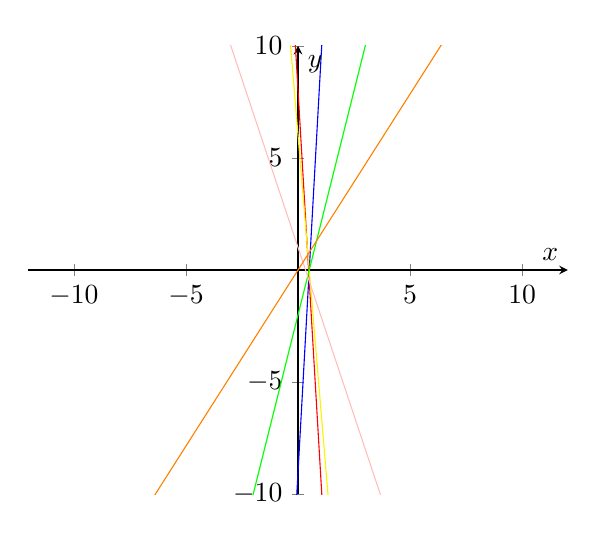
\begin{tikzpicture}
    \begin{axis}[xlabel=$x$,ylabel=$y$,
    xmin=-10,xmax=10,ymin=-10,ymax=10, axis lines=center, axis equal]
        \addplot[domain=-10:10, color=blue,]{18*x-9};
        \addplot[domain=-10:10, color=red,]{-17*x+8};
        \addplot[domain=-10:10, color=yellow,]{-12*x+6};
        \addplot[domain=-10:10, color=green,]{4*x-2};
        \addplot[domain=-10:10, color=pink,]{-3*x+1};
        \addplot[domain=-10:10, color=orange,]{pi/2*x};
    \end{axis}
\end{tikzpicture}

\end{document}